% Drawing 79/15-10 -- folder 79, batch 15, archive page 286 (PDF page 287).
% Transcription: une étoile de six triangles autour d'un sommet.
% Kind: star of six triangles around a vertex. Method 2 (schematic redraw from the facsimile). Status: partial.
% Notes: Six triangles around a vertex: six spokes and the outer hexagon, every stroke drawn with gaps at the vertices. Schematic: outer vertices by eye (the strokes are curved and do not meet).
% Coordinates: 1 unit = 1 mm = 1/100 of the crop width (bbox in page fractions: [0.08, 0.51, 0.25, 0.64]).
% Redrawn by Claude (claude-opus-5-5), issue #73, 2026-11-07; not checked by a human; not compiled (no TeX in the session).
% Rights: reproduces part of the work -- behind RENDER_TRANSCRIPTS, never published by itself.
\documentclass[tikz,border=3pt]{standalone}
\usepackage{amsmath,amssymb}
\usetikzlibrary{patterns,arrows.meta}
\tikzset{pencil/.style={black!45}, struck/.style={black!35}, mark/.style={circle,draw,inner sep=1.3pt}, pt/.style={circle,fill,inner sep=0.9pt}, opt/.style={circle,draw,fill=white,inner sep=1.1pt}}
\begin{document}
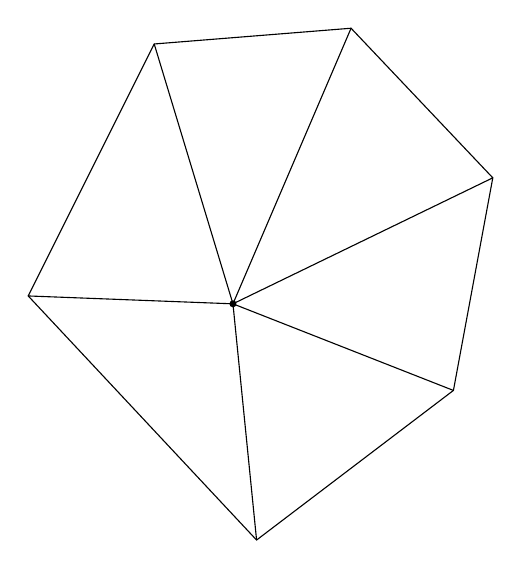
\begin{tikzpicture}[x=1mm,y=1mm,line cap=round,line join=round,font=\scriptsize]
\draw (42,-30) -- (67,-28) -- (85,-47) -- (80,-74) -- (55,-93) -- (26,-62) -- cycle;
\draw (52,-63) -- (42,-30);
\draw (52,-63) -- (67,-28);
\draw (52,-63) -- (85,-47);
\draw (52,-63) -- (80,-74);
\draw (52,-63) -- (55,-93);
\draw (52,-63) -- (26,-62);
\node[pt] at (52,-63) {};
\end{tikzpicture}
\end{document}
